\chapter{An alternative approach to sense-plan-act}
\label{ch:sense-plan-act}
In the following two different control strategy are compared: the \emph{sense-plan-act} and the \emph{task-skill-motion}. Pro and cons of the two approaches are compared to justify the choices made in the work presented in this thesis.

\section{Sense-plan-act}
\graffito{Although this may seems the fastest and simpler approach, on a long-term period causes many redundant and bug-prone re-implementation of the same patterns.}A common approach to control is to solve the overall complex problem by combining the low-level functionalities of the underlying platform into a monolithic control loop, resulting in a controller is strictly tied to that specific problem and therefore poorly re-usable\graffito{Sometimes it is more convenient to re-implement from scratch then re-use old (maybe well-tested!) solutions...}.\\
From a long-term prospective, it is wider to spend more time during the development to come out with a scalable solution for the future.

\section{Task-skill-motion}
Although sense-plan-act is the most widely used control strategy, other alternatives have been proposed. As in MDE we use different DSL's to represent the behavior of the system to be controlled at different levels of abstraction, we can in the same way define multiple control loops, one for every level of behavior abstraction. In many complex application is usually present a mission composed by more task. Each task can be realized employing the skills of the platform and each skill if archived by low-level motion control.\\
\begin{wrapfigure}{r}{0.5\textwidth} %this figure will be at the right
	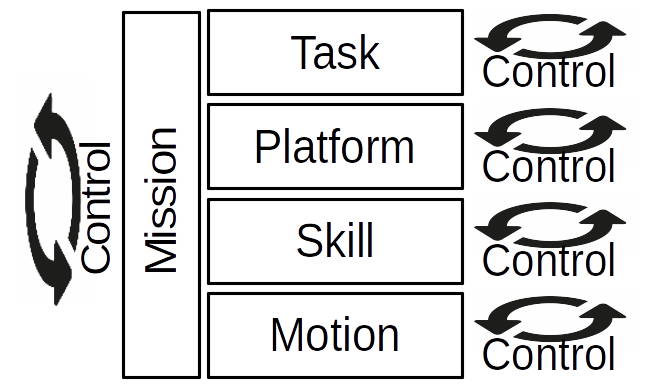
\includegraphics[width=0.7\textwidth]{taskSkillMotion}
	\caption{The task-skill-motion control strategy.}
	\label{fig:taskSkillMotion}
\end{wrapfigure}
We can see that the mission is a far more abstract control problem than the low-level actuation: a mission can be coordinated by a software or human supervisor, usually with more relaxed time constraints, and may distribute the necessary tasks to more agents. Each agent may than decide how to complete the task autonomously, on the basis of its own skills (which obviously depend on the actual hardware platform on which the agent is running). In turn, the skills are composed by one ore more low-level motions.\\
